\chapter{Релейный конструктор}

\section{Выключатели и двоичная логика}

Первые компьютеры были построены на электромагнитных реле. А реле --- это управляемый электрическим
сигналом контакт. То есть это такие переключатели (вроде выключателей света, которыми мы пользуемся дома),
но управляемые не нажатием вручную, а с помощью электрического сигнала.

Выключатели и электрический ток в проводах очень хорошо подходят для работы с двоичным кодом.
Кнопка нажата --- значит $1$, а не нажата --- $0$. Ток течёт --- $1$, не течёт --- $0$.

Например, если на стене расположены $4$ выключателя, то с их помощью
можно закодировать четырёхбитное число. Переключив их в нужные положения
мы <<запишем>> четырёхбитное число. А посмотрев на лампочки,
соединённые с выключателями (условимся, что на выключатели смотреть нельзя),
мы можем узнать, что было записано.
А если на лампочки посмотрит наш друг с другого конца комнаты, то это будет
не просто считывание данных, но ещё и передача их на другое <<устройство>>.

Получается, что запоминать и считывать данные мы можем. А как проводить вычисления?
Хотя бы самые простые логические операции.

Например, мы хотим выполнять логическое <<и>> ($A\ and\ B$): если два выключателя нажаты,
то лампочка загорается, а если хотя бы один разомкнут, лампочка гаснет.
Значит операндами являются состояния выключателей (нажаты или нет),
а результатом состояние лампочки (горит или нет).
Этого можно достичь с помощью последовательного соединения:

\begin{center}
\includegraphics{schemes/switches_and.png}
\end{center}

Слева на схеме источник напряжения, а справа <<земля>>, которая где-то за пределами рисунка
соединена с минусовым контактом источника напряжения.
Если ток будет течь слева направо через всю цепь,
от плюса к минусу, он заставит светиться лампочку <<Результат>>.
Но ток потечёт, если только оба выключателя <<Операнд 1>> и <<Операнд 2>>
будут замкнуты. Если незамкнутым выключателям сопоставить $0$, а замкнутым $1$,
то мы получим, что эта схема выполняет функции логического <<и>>.

Логическое <<или>> ($A\ or\ B$) тоже сделать легко. Ведь ток должен течь
в цепи если любой из выключателей-операндов нажат.
Тогда мы сможем достичь такого результата соединив их параллельно:

\begin{center}
\includegraphics{schemes/switches_or.png}
\end{center}

А что будет, если мы захотим объединить несколько операций в одной схеме?
Например, выход со схемы <<или>> подать на вход схемы <<и>>
(то есть, хотим посчитать что-то вроде $(A\ or\ B)\ and\ C$).
Так как выход у нас это лампочка, а вход --- выключатель,
то придётся поставить туда человека, который будет смотреть на лампочку
и нажимать на нужный выключатель в следующей схеме.

Вот если бы лампочка сама могла <<нажимать>> на выключатель\ldots{ }
И это действительно возможно, только вместо лампочки нужно взять
электромагнит. Так мы сделаем электромагнитное реле.

\section{Электромагнитное реле}

Электромагнитное реле --- это электромагнит, один или несколько
переключателей и якорь (подвижная часть для передачи усилия на переключатели).
При прохождении тока через обмотку электромагнита он
притягивает якорь и нажимает на выключатели. С помощью этого
механизма можно передавать сигналы с выхода одной схемы на вход
другой.

На рисунке ниже схема, в которой есть одно реле (большой прямоугольник).
Внутри этого реле находится электромагнит (перечёркнутый прямоугольник)
и переключаемый контакт. К электромагниту подключена кнопка,
позволяющая подавать на него напряжение, а к переключаемому контакту реле
подключена лампочка.

\begin{center}
\includegraphics{schemes/simple_relay_off.png}
\end{center}

Когда кнопка не нажата, ничего не происходит. Ток не течёт ни через обмотку
электромагнита, ни через лампочку. Если же кнопку нажать, на электромагните
окажется напряжение и он притянет якорь и подвижную часть контакта, замкнув его.
Таким образом цепь с лампочкой тоже замкнётся и лампочка загорится.

\begin{center}
\includegraphics{schemes/simple_relay_on.png}
\end{center}

Когда логические операции реализуются при помощи электромагнитных реле,
в качестве логической единицы обычно используется
наличие напряжения и протекание тока (цепь замкнута),
а для логического нуля --- отсутствие напряжения (цепь разомкнута).

%%%%%%%%%%%%%%%%%

В конструкторе применяются электромагнитные реле с четырьмя
переключающими контактами. Чаще всего в схемах электромагнит и переключающие
контакты изображаются отдельно (как на следующем рисунке слева).
Это может быть удобно, если управляющая цепи и управляемая не связаны
между собой электрически (для этого обычно и нужны реле).

Мы же будем использовать более наглядное обозначение (оно приведено справа на следующем рисунке),
когда и электромагнит и контакты объединяются одним прямоугольником. Это оправданно ещё и тем,
что в наших схемах контакты и катушка зачастую включены в одну цепь.

\begin{center}
\includegraphics{schemes/one_relay.png}
\end{center}

Контакты $13$ и $14$ подключены к катушке, управляющей состоянием контактов.
Когда напряжение на катушку не подано (и ток через неё не течёт),
контакты переключателей соединены так: $9-1$, $10-2$, $11-3$, $12-4$.

Если же реле включится, подвижная часть контактов сдвинется, разомкнув цепи,
описанные выше, и замкнув следующие: $9-5$, $10-6$, $11-7$, $12-8$.

В каждое реле конструктора встроен светодиод, поэтому можно легко увидеть,
когда оно включается. Это помогает отлаживать схемы или наблюдать
хранящиеся в релейной памяти значения.

Во всех модулях параллельно каждой из катушек реле подключён диод в обратном
направлении. Это сделано для предотвращения искрения контактов других реле
(в цепи которых подключена катушка) при их размыкании.
Искрение возникает из-за того, что несмотря на разрыв цепи из-за индуктивности катушки
ток должен продолжать течь какое-то время. Но из-за разрыва это невозможно
в обычном режиме, поэтому возникает электрическая дуга, постепенно разрушающая контакты.

\begin{center}
\includegraphics{schemes/diode.png}
\end{center}

На рисунке подверженный искрению контакт --- это переключатель слева. Он может быть
сам по себе, а может и принадлежать какому-то другому реле.
Чтобы контакты этого переключателя меньше портились и нужен диод.
Оставшийся электрический импульс проходит
уже через него, а не через разомкнутые контакты.

\section{Модули}

Релейный конструктор --- это не просто реле и провода, как можно было бы подумать,
а несколько видов готовых модулей, выполняющих простые функции.
Каждый модуль состоит из печатной платы, нескольких разъёмов на ней
и других компонентов, в зависимости от его функций (реле, переключатели, диоды, резисторы).

С готовыми модулями работать намного удобнее, чем с отдельными диодами, реле и резисторами,
которые ещё нужно чем-то соединить.
Модули похожи на простые микросхемы: один складывает числа, другой
хранит несколько битов информации, и так далее. Ещё есть модуль с переключателями,
чтобы человек мог управлять схемой.

В следующих главах мы будем постепенно знакомиться с каждым из модулей, соединять их друг с другом,
чтобы делать вычислительные устройства: несложные логические схемы, игрушки, калькулятор и в конце концов компьютер.

\section{Соединительные разъёмы}

Модули соединяются между собой с помощью разъёмов на краях плат, как детали конструктора.
Обычно неподалёку от каждого их таких разъёмов находятся ещё и парные им разъёмы для плоских кабелей.
Ими можно воспользоваться, чтобы соединить два модуля, которые не получается состыковать иначе.

В каждом разъёме для подключения платы или кабеля есть контакты для питающего напряжения
(контакт~$1$) и нуля (контакт~$8$).
Поэтому все разъёмы электрически совместимы друг с другом, но логически их соединение не всегда
имеет смысл.

Если какой-то разъём не используется для передачи данных,
к нему можно подключить источник питания. А остальные модули запитаются за счёт того,
что контакты питающего напряжения и нуля есть во всех разъёмах.

Кроме питающего напряжения через соединения передаются и полезные сигналы, занимающие до четырёх контактов
(номера от~$2$ до~$5$), в зависимости от назначения модуля.
Они используются для кодирования четырёхбитного числа или передачи четырёх
управляющих сигналов разного назначения.

Контакты $6$ и $7$ в текущей версии конструктора не используются.


\section{Модуль переключателей}


Модуль с переключателями (или тумблерами) используется для установки
уровней $0$ или $1$ на выходном разъёме вручную.
Присоединяя его к разъёмам других модулей, можно подавать им на вход четырёхбитное число,
либо переключать до четырёх управляющих сигналов.

\begin{center}

\includegraphics{schemes_components/switches.png}
\end{center}

Реализована эта схема в виде такой печатной платы:

\begin{center}
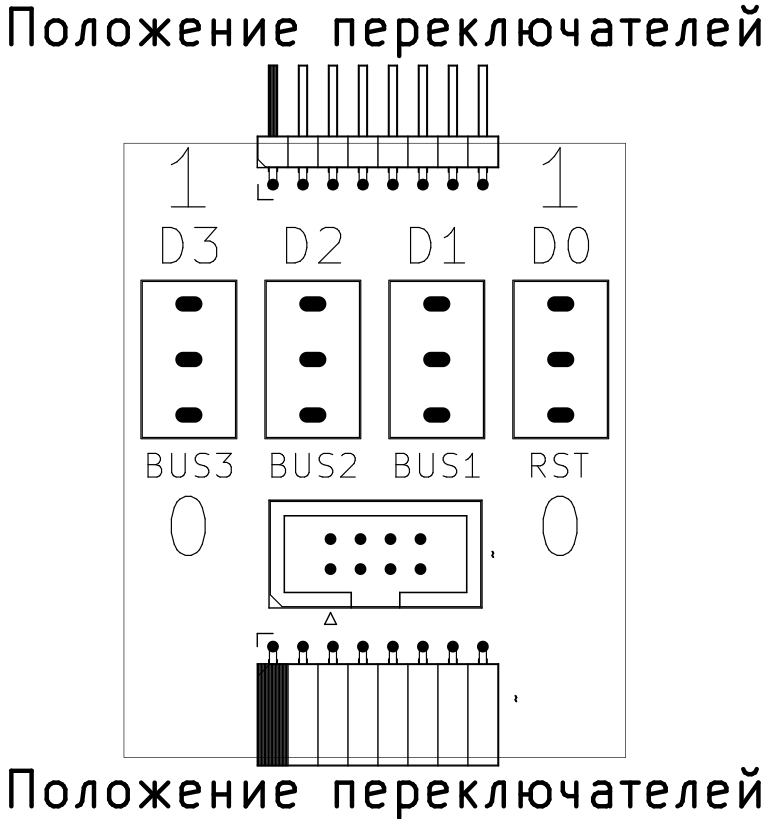
\includegraphics{boards/switches.png}
\end{center}

Входных разъёмов у модуля с тумблерами нет, ведь никакие данные в него не поступают,
чтобы переключить реле или зажечь светодиод. Ведь на плате ничего этого нет.
Поэтому у модуля есть только выходные разъёмы, на которые попадают сигналы
с тумблеров. Одноимённые контакты этих разъёмов соединены между собой. Можно синхронно управлять
одним набором переключателей сразу несколькими модулями, если задействовать нужное количество
выходных разъёмов модуля переключателей.


\section{Практикум}

Проще всего проверить работу тумблеров, подключив их к модулю унарных логических операций.

Список модулей:
\begin{itemize}
    \item Модуль переключателей: $1$ штука
    \item Модуль унарных логических операций: $1$ штука
    \item Проводной шлейф для соединения модулей: $1$ штука
\end{itemize}

Сначала соберём следующую схему.

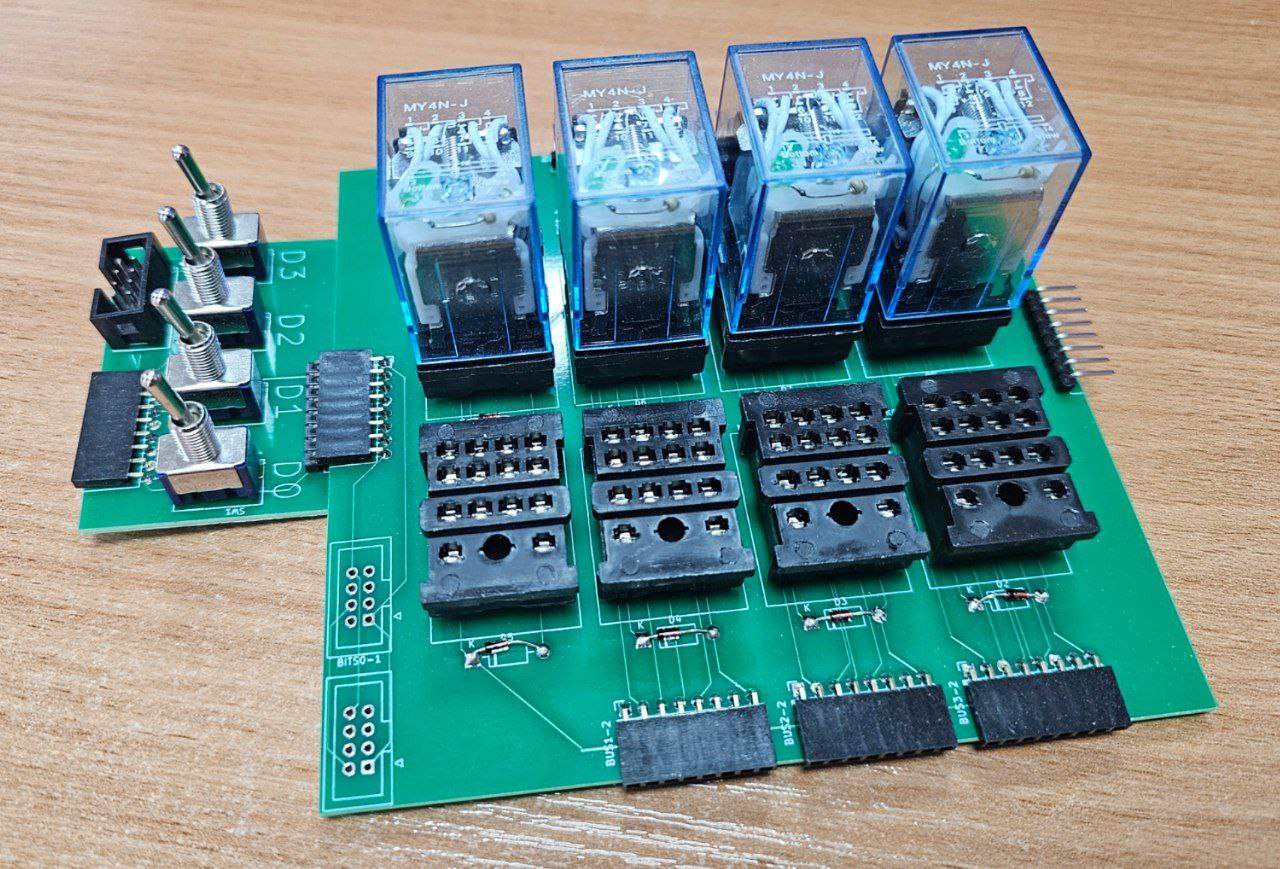
\includegraphics[width=0.5\columnwidth]{photo/switches.jpg}

Источник напряжения можно подключить к любому незадействованному разъёму, потому что
контакты для питания схемы есть на всех разъёмах.

Обычно подключать источник питания нужно последним, но если нужно переставить какой-то
модуль в другое место или добавить какой-то проводник, то можно это делать
и при подключённом питании. Ничего не сломается.

\begin{enumerate}
    \item Попереключайте тумблеры. Убедитесь, что положение одного тумблера меняет состояние одного реле.
    \item Запомните включенное и выключенное состояния тумблеров, а также их порядок по отношению к реле,
          чтобы позднее не было проблем с управлением другими схемами.
\end{enumerate}

Как видите, реле переключаются, в зависимости от положений тумблеров.
При этом реле ещё и генерируют выходные сигналы, но с ними мы поработаем позднее.

Теперь заменим прямое соединение двух плат на соединение с помощью плоского кабеля.

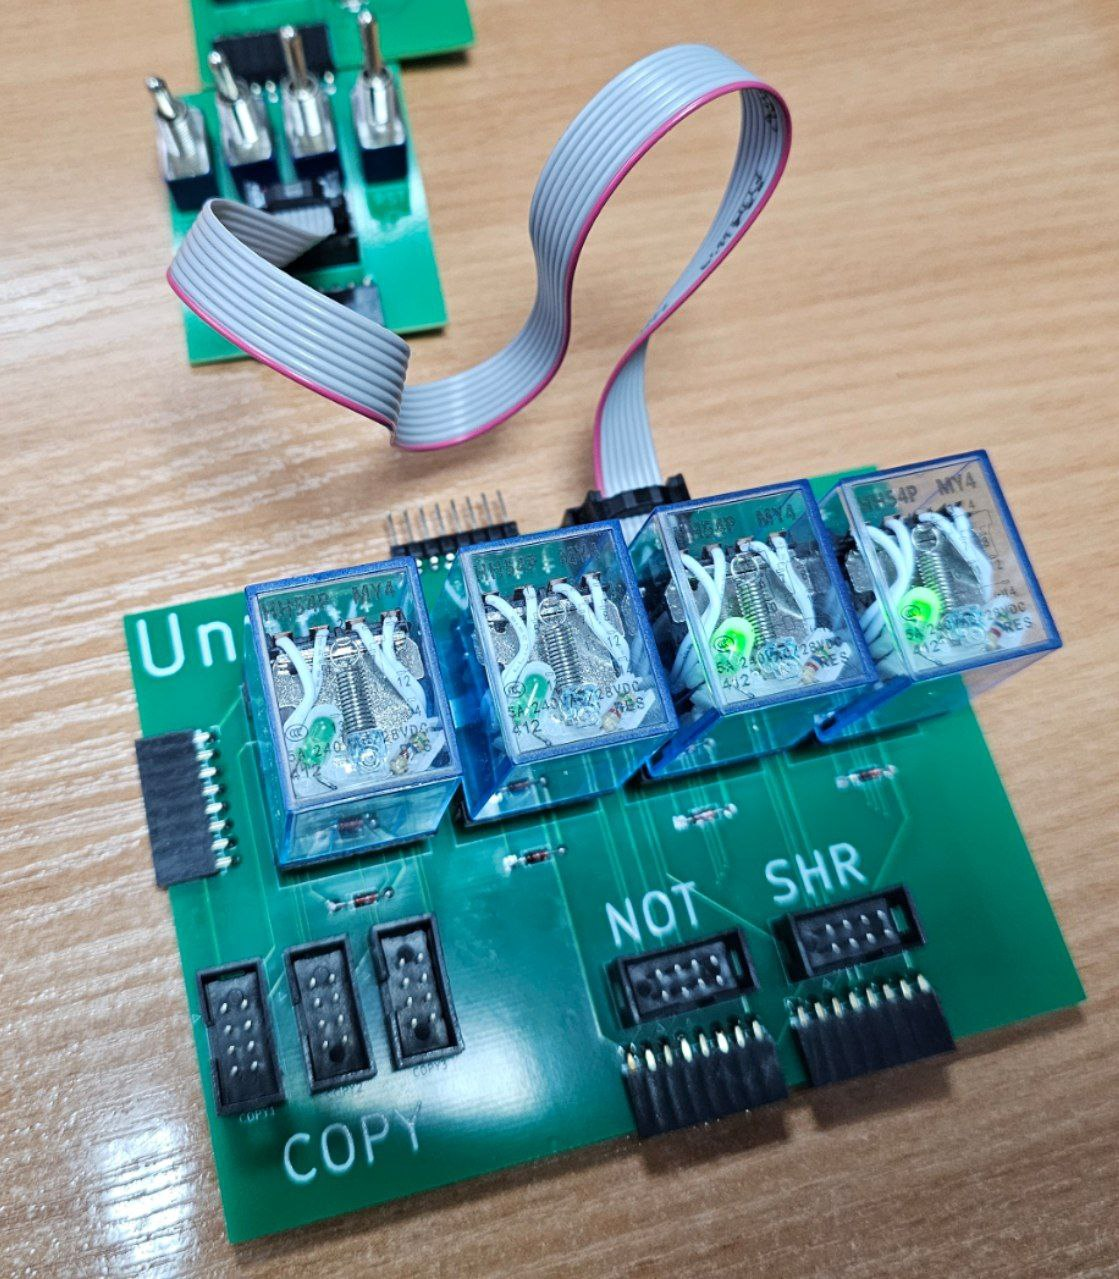
\includegraphics[width=0.5\columnwidth]{photo/switches2.jpg}

Попереключайте тумблеры как раньше, чтобы убедиться, что всё работает ровно так же.
Поэтому дальше выбирайте тот способ подключения, который будет вам удобнее --- они равнозначны.

\section{Задачи}

\begin{enumerate}
    \item Придумайте, как соединить два модуля с тумблерами для выполнения логического ИЛИ.
    % \item Придумать, как соединить тумблеры для выполнения логического И.
\end{enumerate}
